%% LyX 1.2 created this file.  For more info, see http://www.lyx.org/.
%% Do not edit unless you really know what you are doing.
\documentclass[english]{amsart}
\usepackage[T1]{fontenc}
\usepackage[latin1]{inputenc}
\usepackage[dvips]{graphicx}

\makeatletter

%%%%%%%%%%%%%%%%%%%%%%%%%%%%%% LyX specific LaTeX commands.
\providecommand{\LyX}{L\kern-.1667em\lower.25em\hbox{Y}\kern-.125emX\@}

%%%%%%%%%%%%%%%%%%%%%%%%%%%%%% Textclass specific LaTeX commands.
 \theoremstyle{plain}    
 \newtheorem{thm}{Theorem}[section]
 \numberwithin{equation}{section} %% Comment out for sequentially-numbered
 \numberwithin{figure}{section} %% Comment out for sequentially-numbered
 \theoremstyle{plain}    
 \newtheorem{algorithm}[thm]{Algorithm} %%Delete [thm] to re-start numbering
 \usepackage{verbatim}
 \theoremstyle{plain}    
 \newtheorem{cor}[thm]{Corollary} %%Delete [thm] to re-start numbering
 \theoremstyle{plain}    
 \newtheorem{lem}[thm]{Lemma} %%Delete [thm] to re-start numbering
 \theoremstyle{plain}    
 \newtheorem{prop}[thm]{Proposition} %%Delete [thm] to re-start numbering

%%%%%%%%%%%%%%%%%%%%%%%%%%%%%% User specified LaTeX commands.
\newcommand{\R}{{\sf R\hspace*{-0.9ex}\rule{0.15ex}%
       {1.3ex}\hspace*{0.9ex}}}
\newcommand{\N}{{\sf N\hspace*{-1.0ex}\rule{0.15ex}%
       {1.1ex}\hspace*{1.0ex}}}
\newcommand{\Q}{{\sf Q\hspace*{-1ex}\rule{0.15ex}%
       {1.3ex}\hspace*{1.1ex}}}
\newcommand{\C}{{\sf C\hspace*{-0.9ex}\rule{0.15ex}%
       {1.3ex}\hspace*{0.9ex}}}
\usepackage{epsfig}
\usepackage{amsmath,amssymb}
\usepackage{pslatex}
\usepackage{color}


\newif \ifpdf
    \ifx \pdfoutput \undefined
        \pdffalse
    \else
        \pdftrue
\fi


\ifpdf
 \usepackage{thumbpdf}
 \usepackage[pdftex,urlcolor=black,colorlinks=false]{hyperref}
 \pdfinfo{
            /Title      (A family of 4-points dyadic high resolution subdivision schemes)
            /Author     (Daniel Lemire, Ph.D.)
            /Subject 	( By using temporary placeholders on a dense grid, we generalize the 4-point dyadic cubic Deslauriers-Dubuc scheme. Interpolated values require 2 steps to stabilize as they are first interpolated on a coarse scale through a tetradic filter and then on a finer scale using a dyadic filter. The interpolants are C^{1} and can be chosen to reproduce polynomials of degree 4. These generalized interpolatory subdivision schemes have minimal support and no additional memory requirement. This work has applications in CAGD and wavelet theory.)
            /Keywords   (subdivision schemes, interpolation, CAGD, wavelets)
          }

\else
    \usepackage[ps2pdf]{hyperref}
\fi

\topmargin  = 0pt
\headheight = 0pt
\headsep    = 0pt

\voffset    = 0in
\hoffset    = 0in
\textheight = 230mm
\textwidth  = 164mm

\evensidemargin = 0pt
\oddsidemargin  = 0pt

\pagestyle{empty}
\usepackage{float}

\definecolor{veryblackblue}{rgb}{0.0,0.0,0.1}

%% Background of blue palette
 \definecolor{webblackblue}{rgb}{0.0,0.0,0.2}
 \definecolor{webblue}{rgb}{0.0, 0.0, 0.6}

%% Background of red palette
 \definecolor{webblackred}{rgb}{0.2,0.0,0.0}
 \definecolor{webred}{rgb}{0.6,0.0,0.0}

%% Background of green palette
 \definecolor{webblackgreen}{rgb}{0.0,0.2,0.0}                                   
 \definecolor{webgreen}{rgb}{0.0,0.6,0.0} 

%% Background of magenta palette
 \definecolor{webblackmagenta}{rgb}{0.14,0.0,0.14}                                   
 \definecolor{webmagenta}{rgb}{0.42,0.0,0.42} 

%% Background of cyan palette
 \definecolor{webblackcyan}{rgb}{0.0,0.14,0.14}                                   
 \definecolor{webcyan}{rgb}{0.0,0.42,0.42} 

%% Background of yellow pallete
 \definecolor{webblackyellow}{rgb}{0.14,0.14,0.0}                                   
 \definecolor{webyellow}{rgb}{0.85,0.85,0.0} 

 \definecolor{webdarkgray}{rgb}{0.2,0.2,0.2}

 \definecolor{webgray}{rgb}{0.75,0.75,0.75}
 \definecolor{weborange}{rgb}{1.0, 0.6, 0.0}

\renewcommand\labelenumi{\textcolor{webdarkgray}{\arabic{enumi}.}}
\newcommand{\setenumi}[1]{#1.\setcounter{enumi}{#1}}
\usepackage{dsfont}
%\newcommand{\Z}{\mathds{Z}}
\newfont{\first}{msbm10 at 12pt}
\newcommand{\Z}{\mbox{\first{Z}}}
\usepackage{pstricks}

\makeatother
\usepackage{babel}
\begin{document}

\title{A Family of 4-point Dyadic High Resolution Subdivision Schemes}


\author{Daniel Lemire}

\begin{abstract}
We present a new family of multistep iterative interpolation schemes
generalizing subdivision schemes so that quartic polynomials can be
reproduced with a $4-$point approach. Interpolation requires two
steps: a coarse scale interpolation followed by a fine scale interpolation.
The interpolants are $C^{1}$, have good local properties and no additional
memory requirement.
\end{abstract}

\keywords{Subdivision Schemes, Fourier transform, CAGD, Wavelets, Lagrange
Interpolation, Richardson Extrapolation}

\maketitle

\section{Introduction}

Interpolatory subdivision schemes interpolate a discrete set of data
points in a local manner, that is, the value of the interpolation
function at a given point depends on a small number of nearby data
points. The classical dyadic algorithm \cite{Du,DeDu} finds the midpoint
values by fitting a Lagrange polynomial through the $2N$ closest
data points. By repeating this algorithm again and again, each time
doubling the number of data points or nodes by midpoint interpolation,
we eventually have a dense set of data points and can determine uniquely
a smooth interpolation function. Because interpolatory subdivision
schemes relate data points from one scale to another scale, it is
not surprising that they are a key ingredient in the construction
of compactly supported wavelets \cite{Dau,DeDuLe}.

More recently, Merrien \cite{Me92,Me99,DuLeMe} introduced Hermite
subdivision schemes. Since Merrien subdivision schemes use Hermite
nodes, they have have twice the approximation order and better regularity
for a given support. For example, $2-$point Hermite schemes are differentiable
and can reproduce quadratic or cubic polynomials whereas the corresponding
$2-$point Deslauriers-Dubuc scheme (the linear spline) is not differentiable
and only reproduces linear polynomials.

Therefore, we propose to add intermediate nodes to Deslauriers-Dubuc
schemes and subdivision schemes in general to improve approximation
and local properties. Adding extra nodes to improve an interpolation
scheme is not a new approach and has been used to make spline interpolation
local \cite{DuGe}. However, doubling the number of nodes doubles
the memory requirements. On the other hand, dyadic subdivision scheme
double their memory usage at each step. Hence, we can choose to use
one step earlier the upcoming extra storage space without any cost.
These new intermediate nodes or placeholders can then be used to record
a coarse scale guess (using a tetradic filter) which we can later
combine with a finer scale interpolation (using a dyadic filter).
These schemes are said to be {}``high resolution'' because we no
longer consider only the next finer scale, but actually the next two
finer scales; alternatively, we could describe these algorithms as
{}``two-step subdivision schemes''. Whereas subdivision schemes
immediately fix the interpolated value, we choose to only record the
interpolated values as {}``reasonable guesses'' and allow to scheme
to correct the guess later based on the results at finer scales.

The main result of this paper is that by summing up the tetradic (coarse)
interpolation recorded in placeholders and dyadic (fine) interpolations,
we get a range of smooth ($C^{1}$) high resolutions schemes reproducing
at least cubic polynomials. It is also shown that whereas $4-$point
subdivision scheme can reproduce at most cubic polynomials, $4-$point
high resolution subdivision (HRS) schemes can reproduce quartic polynomials
(see Table \ref{cap:Comparaison-between-some}).

The paper is organized as follows. We begin by a brief review of subdivision
schemes and give explicit algorithms for both the dyadic and tetradic
$4-$point Deslauriers-Dubuc schemes. Combining these subdivision
schemes, we present a family of HRS schemes and show that this new
family can reproduce cubic and even quartic polynomials. We conclude
by proving that some of these schemes are smooth ($C^{1}$).\begin{figure} \centering % PSTricks TeX macro
% Title: Untitled-1
% Creator: Dia v0.88.1
% CreationDate: Thu May 23 16:50:34 2002
% For: lemire
% \usepackage{pstricks}
% The following commands are not supported in PSTricks at present
% We define them conditionally, so when they are implemented,
% this pstricks file will use them.
\ifx\setlinejoinmode\undefined
  \newcommand{\setlinejoinmode}[1]{}
\fi
\ifx\setlinecaps\undefined
  \newcommand{\setlinecaps}[1]{}
\fi
% This way define your own fonts mapping (for example with ifthen)
\ifx\setfont\undefined
  \newcommand{\setfont}[2]{}
\fi
\pspicture(6.111818,-9.988182)(11.688182,-5.261818)
\scalebox{1.000000 -1.000000}{
\newrgbcolor{dialinecolor}{0.000000 0.000000 0.000000}
\psset{linecolor=dialinecolor}
\newrgbcolor{diafillcolor}{1.000000 1.000000 1.000000}
\psset{fillcolor=diafillcolor}
\psset{linewidth=0.100000}
\psset{linestyle=solid}
\psset{linestyle=solid}
\setlinecaps{0}
\newrgbcolor{dialinecolor}{0.000000 0.000000 0.000000}
\psset{linecolor=dialinecolor}
\psclip{\pswedge[linestyle=none,fillstyle=none](5.036504,3.055273){9.876956}{18.748036}{80.825962}}
\psellipse(5.036504,3.055273)(6.984062,6.984062)
\endpsclip
}\endpspicture \caption{A caption} \label{figure:alabel} \end{figure} 

\begin{figure*}%

\caption{fd}\end{figure*}%


\begin{table}%
\begin{center}\begin{tabular}{|c|c|c|c|}
\hline 
scheme&
regularity&
number of samples at step $j$&
reproduced polynomials\\
\hline
\hline 
Dubuc\cite{Du}&
$C^{1}$&
$2^{j}N$&
cubic\\
\hline 
Deslauriers-Dubuc\cite{DeDu}&
$C^{1}$&
$b^{j}N$&
cubic\\
\hline 
Dyn-Gregory-Levin\cite{DyGrLe}&
up to $C^{1}$&
$2^{j}N$&
up to cubic\\
\hline 
Hassan et al.\cite{HaIvDoSa}&
$C^{2}$&
$3^{j}N$&
quadratic\\
\hline 
presented HRS&
up to $C^{1}$&
$2^{j+1}N$&
tetradic\\
\hline
\end{tabular}\end{center}


\caption{\label{cap:Comparaison-between-some}Comparaison between some $4-$point
iterative interpolation schemes.}\end{table}%



\section{Subdivision schemes}

Let $b>1$ be an integer, given two integers $k,j$, the number $x_{j,k}=k/b^{j}$
is said to be $b-$adic (of depth $j$). For a fixed $j$, the $b-$adic
numbers form a regularly spaced set of nodes. For a fixed $J$, given
some data $\left\{ y_{J,k}\right\} _{k\in \Z }$, we want a smooth
function $f$ such that $f\left(x_{J,k}\right)=y_{J,k}\, \forall k\in \Z $.
Starting with ($y_{J,k}$) and using the formula \begin{equation}
y_{j+1,l}=\sum _{k\in \Z }\gamma _{bk-l}y_{j,k}\label{basicsubdivision}\end{equation}
 for some array $\gamma $, we get values $y_{j,k}$ for any $j>J$
and since $b-$adic numbers form a dense set in $\R $, there is at
most one continuous function such that $f\left(x_{j,k}\right)=y_{j,k}$
for all $k\in \Z ,j>J$. 

A subdivision scheme is \textit{interpolatory} and satisfies $f\left(x_{J,k}\right)=y_{J,k}$
if $\gamma _{bk}=0\, \forall k\in \Z $ except for $\gamma _{0}=1$.
We say that a subdivision scheme is \textit{stationary} if the array
$\gamma $ is constant (does not depend on $j$). Because $\gamma $
does not depend explicitely on $l$ but rather on $bk-l$ the scheme
is \textit{translation invariant} or \textit{homogeneous}. A subdivision
scheme is $2N-$point if $\gamma _{l}=0$ for $|l|>Nb$. The fundamental
function of an interpolatory $2N-$point $b-$adic scheme has initial
data $y_{0,0}=1$ and $y_{0,k}=0$ for all $k\neq 0$; it has a compact
support of $[-(Nb-1)/(b-1),(Nb-1)/(b-1)]$ (or $[1-2N,2N-1]$ when
$b=2$). 

For $N=1,2,3,...$ there are corresponding interpolatory $2N-$point
interpolatory Deslauriers-Dubuc subdivision schemes built from the
midpoint evaluation of Lagrange polynomial of degree $2N-1$. For
$b=2$ (dyadic case), the $4-$point Deslauriers-Dubuc scheme can
be defined with the array $\gamma ^{DD2}$ given by $\gamma _{0}^{DD2}=1,\, $$\gamma _{1}^{DD2}=\gamma _{-1}^{DD2}=-9/16,\, $$\gamma _{3}^{DD2}=\gamma _{-3}^{DD2}=-1/16$
with $\gamma _{k}^{DD2}=0$ otherwise; for $b=4$ (tetradic case),
the scheme is defined with the array $\gamma ^{DD4}$ given by $\gamma _{2k}^{DD4}=\gamma _{k}^{DD2}\, \forall k\in \Z ,\, $
$\gamma _{-1}^{DD4}=\gamma _{1}^{DD4}=105/128,\, $$\gamma _{-3}^{DD4}=\gamma _{-3}^{DD4}=35/128,\, $$\gamma _{-5}^{DD4}=\gamma _{5}^{DD4}=-7/128,\, $$\gamma _{-7}^{DD4}=\gamma _{7}^{DD4}=-5/128,\, $with
$\gamma _{k}^{DD2}=0$ otherwise. 

Because $4-$point Deslauriers-Dubuc schemes are derived from cubic
Lagrange polynomials, they reproduce cubic polynomials, that is, if
the initial data $y_{j,k}$ satisfies $y_{j,k}=p\left(x_{j,k}\right)\, \forall k\in \Z $
for some cubic polynomial $p$ then the interpolation function $f$
is this same cubic polynomial $f=p$. The two cases presented above
($\gamma ^{DD2}$ and $\gamma ^{DD4}$) reproduce cubic polynomials
and they both converge to differentiable ($C^{1}$) interpolation
functions. Because we later borrow from these two subdivision schemes,
we give explicit algorithms for both schemes.

\begin{algorithm}
($4-$point Deslauriers-Dubuc Dyadic Scheme) For a given integer $j$,
begin with some initial $y-$values $y_{j,k}\, k\in \Z $ over dyadic
numbers $x_{j,k}=k/2^{j}$,
\begin{enumerate}
\item recopy data at $x_{j+1,2k}=x_{j,k}$: $y_{j+1,2k}=y_{j,k}\, \forall k\in \Z $
;
\item interpolate midpoint value by the corresponding cubic Lagrange polynomial:
\[
y_{j+1,2k+1}=\frac{-y_{j,k-1}+9y_{j,k}+9y_{j,k+1}-y_{j,k+2}}{128}\, \forall k\in \Z ;\]

\item Repeat with $j\rightarrow j+1$ and using $y_{j+1}$ as initial data.
\end{enumerate}
\end{algorithm}
~

\begin{algorithm}
($4-$point Deslauriers-Dubuc Tetradic Subdivision Scheme) For a given
integer $j$, begin with some initial $y-$values $y_{j,k}\, k\in \Z $
over $4-$adic numbers $x_{j,k}=k/4^{j}$
\begin{enumerate}
\item recopy data at $x_{j+1,4k}=x_{j,k}$: $y_{j+1,4k}=y_{j,k}\, \forall k\in \Z $
;
\item interpolate quartertile point values by the corresponding cubic Lagrange
polynomial: \[
y_{j+1,4k+1}=\frac{-7y_{j,k-1}+105y_{j,k}+35y_{j,k+1}-5y_{j,k+2}}{128};\]
 \[
y_{j+1,4k+2}=\frac{-y_{j,k-1}+9y_{j,k}+9y_{j,k+1}-y_{j,k+2}}{128};\]
\[
y_{j+1,4k+3}=\frac{-5y_{j,k-1}+35y_{j,k}+105y_{j,k+1}-7y_{j,k+2}}{128}\, \forall k\in \Z ;\]

\item Repeat with $j\rightarrow j+1$ and using $y_{j+1}$ as initial data.
\end{enumerate}
\end{algorithm}

\section{High resolution subdivision schemes}


\subsection{Definitions}

In this paper, we want to extend subdivision schemes by hybrid schemes:
mixing tetradic and dyadic subdivision schemes for example. Given
some data $\left\{ y_{j-1,k}\right\} _{k\in \Z }$ on the dyadic $x_{j-1,k}$
grid, we must apply a dyadic subdivision scheme as an initialisation
step: since HRS schemes can be seen as multistep subdivision schemes,
it is not surprising that they require an initialisation step. For
$4-$point HRS schemes, a sensible choice for the initialization step
is the $4-$point Deslauriers-Dubuc dyadic scheme (see lemma \ref{lemmecubic})
which copies the data at even nodes ($y_{j,2k}=y_{j-1,k}$) and insert
new values ({}``guesses'') at odd nodes ($y_{j,2k+1}$ for $k\in \Z $).
A value $y_{j,k}$ is {}``stable'' if $y_{j,k}=y_{j+1,2k}$ and
other nodes are said to be temporary or are referred to as {}``placeholders''.
A HRS on a dyadic grid is interpolatory if all $y_{j,2k}$ values
on even nodes ($x_{j,2k}$) are stable so that $y_{j,2k}=y_{j+1,4k}\, \forall k\in \Z $.
Assuming we used an interpolatory subdivision scheme as an initialization
step, the following HRS algorithm is interpolatory.

\begin{algorithm}
\label{4pointhrssalgo}($4-$point Dyadic HRS Schemes) The following
iteration steps depend on $\alpha \in \R $, a constant parameter.
For a given integer $j$, begin with some initial $y-$values $y_{j,k}\, k\in \Z $
over dyadic numbers $x_{j,k}=k/2^{j}$ where only the even nodes are
interpolated ($y_{j,2k}$),
\begin{enumerate}
\item recopy stable data: $y_{j+1,4k}=y_{j,2k}\, \forall k\in \Z $ ;
\item Apply the $4-$point Deslauriers-Dubuc tetradic scheme on even (stable)
nodes: \[
y_{j+1,4k+1}=\frac{-7y_{j,2k-2}+105y_{j,2k}+35y_{j,2k+2}-5y_{j,2k+4}}{128};\]
 \[
y_{j+1,4k+2}^{temporary}=\frac{-y_{j,2k-2}+9y_{j,2k}+9y_{j,2k+2}-y_{j,2k+4}}{128};\]
\[
y_{j+1,4k+3}=\frac{-5y_{j,2k-2}+35y_{j,2k}+105y_{j,2k+2}-7y_{j,2k+4}}{128}\, \forall k\in \Z ;\]

\item Update midpoint (which then becomes stable): \[
y_{j+1,4k+2}=(1-\alpha )y_{j+1,4k+2}^{temporary}+\alpha y_{j,2k+1};\]

\item Repeat with $j\rightarrow j+1$ and using $y_{j+1}$ as initial data.
\end{enumerate}
\end{algorithm}
This new algorithm is not a subdivision scheme in general and thus,
we need a more general definition: stationary subdivision schemes
(equation \ref{basicsubdivision}) can be generalized by the linear
equation\begin{equation}
y_{j+1,l}=\sum _{m=1}^{M}\sum _{k\in \Z }\gamma _{Mbk+m-1-l}^{(m)}y_{j,Mk+m-1}\label{hrgeneral}\end{equation}
where $\gamma ^{(1)},...,\gamma ^{(M)}$ are constant arrays (independent
from $j$). It can be said to be $b-$adic because the number of nodes
is increasing by a factor of $b$ with each iteration but because
we have $M>1$ arrays $\gamma $, the scheme is said to be a HRS scheme.
We say it is interpolatory if it satisfies $y_{j+1,Mbk}=y_{j+1,Mk}$
and it is $2N-$point if $\gamma _{l}^{(m)}=0$ for $|l|>MNb$ and
$m=1,...,M$. For $b=M=2$ the general equation \ref{hrgeneral} becomes
\begin{equation}
y_{j+1,l}=\sum _{k\in \Z }\gamma _{4k-l}^{(1)}y_{j,2k}+\gamma _{4k+1-l}^{(2)}y_{j,2k+1}.\label{N2highres}\end{equation}
It is interpolatory if $y_{j+1,4k}=y_{j+1,2k}$ and $2N-$point if
$\gamma _{l}^{(m)}=0$ for $|l|>2Nb$ and $m=1,2$. It should be noted
that for an algorithm based on HRS scheme to be interpolatory, the
initialization step must be interpolatory ($y_{j,bk}=y_{j-1,k}$).

The interpolatory algorithm \ref{4pointhrssalgo} amounts to choosing
$\gamma ^{(1)}$ and $\gamma ^{(2)}$ to be:

\begin{eqnarray}
\gamma _{2k}^{(1)}=\gamma _{2k}^{DD4}+\alpha \left(\delta _{k,0}-\gamma _{k}^{DD2}\right),\,  & \gamma _{2k+1}^{(1)}=\gamma _{2k+1}^{DD4}\, \forall k\in \Z  & \label{N2highres_1}\\
\gamma _{0}^{(2)}=\alpha ,\,  & \gamma _{k}^{(2)}=0\, otherwise & \label{N2highres_2}
\end{eqnarray}
 for some parameter $\alpha \in \R $. Indeed, since $\gamma _{2k}^{DD4}=\gamma _{k}^{DD2}\, \forall k\in \Z $,
we can rewrite equation \ref{N2highres} for even and odd terms. Firstly,
setting $l=2s$ ($l$ even), we have \begin{eqnarray*}
y_{j+1,2s} & =\sum _{k\in \Z } & \gamma _{4k-2s}^{(1)}y_{j,2k}+\gamma _{4k+1-2s}^{(2)}y_{j,2k+1}\\
 & =\sum _{k\in \Z } & \left(\gamma _{4k-2s}^{DD4}-\alpha \gamma _{2k-s}^{DD2}+\alpha \delta _{4k,2s}\right)y_{j,2k}+\alpha \delta _{4k+1,s}y_{j,2k+1}\\
 & =\sum _{k\in \Z } & \left((1-\alpha )\gamma _{2k-s}^{DD2}+\alpha \delta _{2k,s}\right)y_{j,2k}+\delta _{2k+1,s+1}\alpha y_{j,2k+1}
\end{eqnarray*}
so that when $s$ is even ($l=2s=4r$), we have the interpolatory
condition \begin{equation}
y_{j+1,4r}=y_{j,2r}\label{hrsinterpole}\end{equation}
otherwise, when $s$ is odd $(l=2s=4r+2)$\begin{equation}
y_{j+1,4r+2}=\alpha y_{j,2r+1}+(1-\alpha )\sum _{k\in \Z }\gamma _{2k-2r-1}^{DD2}y_{j,2k}.\label{hrsricharson}\end{equation}
Secondly, if $l$ is odd ($l=2s+1$), we have\begin{eqnarray}
y_{j+1,2s+1} & = & \sum _{k\in \Z }\gamma _{4k-2s-1}^{(1)}y_{j,2k}+\gamma _{4k-2s-1}^{(2)}y_{j,2k+1}\nonumber \\
 & = & \sum _{k\in \Z }\gamma _{4k-2s-1}^{DD4}y_{j,2k}.\label{hrswidguess}
\end{eqnarray}
Equations \ref{hrsinterpole}, \ref{hrsricharson}, and \ref{hrswidguess}
can be used to describe the presented HRS schemes: while equation
\ref{hrsinterpole} is the interpolatory condition, equation \ref{hrswidguess}
fills the placeholders with tetradic (coarse scale) interpolated values
whereas equation \ref{hrsricharson} combines the value stored in
the placeholder with the newly available interpolated value (fine
scale) given by the summation term which we recognize from the dyadic
Deslauriers-Dubuc interpolation. 

In the simplest case, $\alpha =0$, equation \ref{N2highres} becomes\begin{equation}
y_{j+1,l}=\sum _{k\in \Z }\gamma _{4k-l}^{DD4}y_{j,2k}.\label{N2highresalpha0}\end{equation}
Because $\alpha =0\Rightarrow \gamma ^{(2)}=0$, we see that the placeholders
(odd nodes) are effectively ignored. Indeed, we observe that this
last equation discards odd nodes at each step: $y_{j+1,l}$ depends
only on even nodes ($y_{j,2k}$ ) and not at all on the odd nodes
( $y_{j,2k+1}$). Hence, we can replace equation \ref{N2highresalpha0}
by \[
y_{j+1,2l}=\sum _{k\in \Z }\gamma _{4k-2l}^{DD4}y_{j,2k}\]
but because $\gamma _{2k}^{DD4}=\gamma _{k}^{DD2}$ , this last equation
becomes $y_{j+1,2l}=\gamma _{2k-l}^{DD2}y_{j,2k}$ and if we define
$\widetilde{y}_{j,k}=y_{j,2k}$ then \begin{equation}
\widetilde{y}_{j+1,2l}=\sum _{k\in \Z }\gamma _{2k-l}^{DD2}\widetilde{y}_{j,2k}\label{DD2}\end{equation}
which we recognize as the cubic Deslauriers-Dubuc scheme and we have
proved the next proposition. 

\begin{prop}
\label{propDesDuequiv}For $\alpha =0$, the HRS scheme given by algorithm
\ref{4pointhrssalgo} is equivalent to the $4-$point dyadic Deslauriers-Dubuc
subdivision scheme.
\end{prop}
Thus we can say that the presented family of HRS schemes generalizes
the dyadic Deslauriers-Dubuc scheme \cite{Du,DeDu}.


\subsection{Local properties}

Not surprisingly, $2N-$point HRS schemes are {}``as local as''
the corresponding $2N-$point subdivision scheme since interpolated
values depend only on the closest $2N$ nodes and we use a dyadic
tree. As an example, consider any $2N-$point dyadic HRS scheme. Since
the algorithm is linear, stationary and homogeneous, we can choose
$y_{0,0}=1$ and $y_{0,k}=0$ for $k\neq 0$ to characterize locality.
As an initialization step, apply any interpolatory $2N-$point dyadic
subdivision scheme: the farthest non-zero interpolated values are
$y_{1,\pm (2N-1)}$ at $\pm \xi _{0}$ where $\xi _{0}=\frac{2N-1}{2}$.
We then apply the $4-$point HRS scheme itself treating the odd nodes
$y_{1,-(2N-1)},...,y_{1,2N-1}$ as placeholders, the farthest non-zero
interpolated values are at $\pm \xi _{1}$ where $\xi _{1}=\xi _{0}+\frac{2N-1}{2^{2}}$:
in this respect, a HRS scheme behaves just like subdivision schemes.
Of course, these farthest values are not stable yet since they are
located at odd nodes, but they become stable at the next interation.
By induction, the farthest non-zero interpolated values after $n$
interations is at $\xi _{n}=\sum _{k=1}^{n}\frac{2N-1}{2^{k}}$ which
converges to $2N-1$ as $n\rightarrow \infty $ and hence, the support
of the interpolated function has to be in $[1-2N,2N-1]$. A similar
argument could be made when $b\neq 2$ (non-dyadic case).

Since the $2N-$point HRS schemes are as local as $2N-$point subdivision
schemes, it remains to show that HRS schemes can {}``outperform''
subdivision schemes in some respect. We begin by showing that for
the presented schemes, the degree of the reproduced polynomials is
at least the same (cubic) and then we proceed to show that we can
do better (quartic).


\subsection{Reproduced polynomials}

Assume that for some $j$, $y_{j,k}=p_{3}\left(x_{j,k}\right)\, \forall k\in \Z $
where $p_{3}$is a cubic polynomial. Because $4-$point Deslauriers-Dubuc
schemes reproduce cubic polynomials, we have \[
\sum _{k\in \Z }\gamma _{2k-2r-1}^{DD2}y_{j,2k}=y_{j,2r+1}=p_{3}\left(x_{j,2r+1}\right)\]
and thus equation \ref{hrsricharson} becomes $y_{j+1,4r+2}=p_{3}\left(x_{j,2r+1}\right)$
for any $\alpha \in \R $. Similarly, equation \ref{hrswidguess}
implies $y_{j+1,2s+1}=p_{3}\left(x_{j+1,2s+1}\right)$. We can conclude
that $y_{j+1,k}=p_{3}\left(x_{j+1,k}\right)\, \forall k\in \Z $ if
$y_{j,k}=p_{3}\left(x_{j,k}\right)\, \forall k\in \Z $ and thus HRS
schemes defined by equation \ref{N2highres} reproduce cubic polynomials.
As we have seen, for practical implementations of a high subdivision
scheme, it is necessary to first apply a one-step subdivision scheme.
This can be solved by a (one-step) dyadic Deslauriers-Dubuc interpolation.
Let $\left\{ y_{j,k}\right\} _{k}$ be some initial data. As a first
step, we apply equation\begin{equation}
y_{j+1,l}=\sum _{k\in \Z }\gamma _{2k-l}^{DD2}y_{j,2k}\label{DD2_2}\end{equation}
 followed by algorithm \ref{4pointhrssalgo} with $j+1$. By induction
on $j$ using algorithm \ref{4pointhrssalgo}, we get the following
lemma.

\begin{lem}
\label{lemmecubic}HRS schemes given by algorithm \ref{4pointhrssalgo}
reproduce cubic polynomials and are interpolatory when using a one
step interpolatory 4-point dyadic Deslauriers-Dubuc interpolation
(equation \ref{DD2_2}) as initialization.
\end{lem}
We can also get a stronger result by choosing a specific $\alpha $.
We can write any quartic polynomial $p_{4}$ as $p_{4}(x)=a_{4}x^{4}+p_{3}(x)$
where $p_{3}$ is some cubic polynomial. Suppose that for some $j$,
$y_{j,2k}=p_{4}\left(x_{j,2k}\right)$ and $y_{j-1,k}=p_{4}\left(x_{j-1,k}\right)\, \forall k\in \Z $.
We can write $y_{j+1,4r+2}$ for any $r\in \Z $ in terms of this
initial data ($y_{j}$ and $y_{j-1}$) by substituting equation \ref{hrswidguess}
into \ref{hrsricharson} to get \begin{eqnarray}
y_{j+1,4r+2} & = & \alpha y_{j,2r+1}+(1-\alpha )\sum _{k\in \Z }\gamma _{2k-2r-1}^{DD2}y_{j,2k}\nonumber \\
 & = & \alpha \sum _{k\in \Z }\gamma _{4k-2r-1}^{DD4}y_{j-1,2k}+(1-\alpha )\sum _{k\in \Z }\gamma _{2k-2r-1}^{DD2}y_{j,2k}.\label{upcomingrichardson}
\end{eqnarray}
We want to show that $y_{j+1,4r+2}=p_{4}\left(x_{j,2r+1}\right)$
for some $\alpha \in \R $ and so we substitute $y_{j,2k}=p_{4}\left(x_{j,2k}\right)$
and $y_{j-1,k}=p_{4}\left(x_{j-1,k}\right)$ into the two sums of
this last equation. Because of the identities \begin{eqnarray*}
\frac{-9}{2^{4j}} & = & \frac{-\left(x_{j,2r-2}\right)^{4}+9\left(x_{j,2r}\right)^{4}+9\left(x_{j,2r+2}\right)^{4}-\left(x_{j,2r+4}\right)^{4}}{128}-\left(x_{j,2r+1}\right)^{4}\\
\frac{-105}{2^{4j}} & = & \frac{-7\left(x_{j,2r-4}\right)^{4}+105\left(x_{j,2r}\right)^{4}+35\left(x_{j,2r+4}\right)^{4}-5\left(x_{j,2r+8}\right)^{4}}{128}-\left(x_{j,2r+1}\right)^{4}\\
 & = & \frac{-5\left(x_{j,2r-4}\right)^{4}+35\left(x_{j,2r}\right)^{4}+105\left(x_{j,2r+4}\right)^{4}-7\left(x_{j,2r+8}\right)^{4}}{128}-\left(x_{j,2r+1}\right)^{4},
\end{eqnarray*}
we can compute both sums in equation \ref{upcomingrichardson} explicitely:
\begin{eqnarray}
\sum _{k\in \Z }\gamma _{4k-2r-1}^{DD4}y_{j-1,2k} & = & p_{3}\left(x_{j,2r+1}\right)+a_{4}\sum _{k\in \Z }\gamma _{4k-2r-1}^{DD4}\times \left(x_{j-1,2k}=x_{j,4k}\right)^{4}\\
 & = & p_{4}\left(x_{j,2r+1}\right)-\frac{105a_{4}}{2^{4j}}\label{105sur16}
\end{eqnarray}
 and\begin{eqnarray*}
\sum _{k\in \Z }\gamma _{2k-2r-1}^{DD2}y_{j,2k} & = & p_{3}\left(x_{j,2r+1}\right)+a_{4}\sum _{k\in \Z }\gamma _{2k-2r-1}^{DD2}\times \left(x_{j,2k}\right)^{4}\\
 & = & p_{4}\left(x_{j,2r+1}\right)-\frac{9a_{4}}{2^{4j}}
\end{eqnarray*}
Hence, setting $\alpha =-3/32$ in equation \ref{upcomingrichardson},
we get \[
y_{j+1,4r+2}=p_{4}\left(x_{j,2r+1}\right)-\frac{105\alpha +9(1-\alpha )}{2^{4j}}a_{4}=p_{4}\left(x_{j+1,4r+2}\right)\]
since for $\alpha =-3/32$, $105\alpha +9(1-\alpha )=0$. Therefore,
the HRS scheme with $\alpha =-3/32$ reproduces quartic polynomials. 

For pratical applications, we may wish to initialize HRS schemes with
an interpolatory subdivision scheme so that the whole process remains
interpolatory. While there are no $4-$point subdivision scheme capable
of interpolating $y_{j-1,k}=p_{4}\left(x_{j,k}\right)$ into $y_{j,2k+1}=p_{4}\left(x_{j,2k+1}\right)-\frac{105a_{4}}{16\times 2^{4j}}$
and $y_{j,2k}=p_{4}\left(x_{j,2k}\right)$ for all $k\in \Z $, there
exist $5-$point subdivision schemes such as the subdivision scheme
described by the next algorithm.

\begin{algorithm}
\label{5pointalgo}($5-$point {}``Initialization'' Subdivision
Scheme) For a given integer $j$, begin with some initial $y-$values
$y_{j,k}\, k\in \Z $ over dyadic numbers $x_{j,k}=k/2^{j}$,
\begin{enumerate}
\item recopy data at $x_{j+1,2k}=x_{j,k}$: $y_{j+1,2k}=y_{j,k}\, \forall k\in \Z $
;
\item extrapolate $y_{j,k+4}$ using $y_{j,k-2},y_{j,k-1},y_{j,k},y_{j,k+1},y_{j,k+2}$
by the formula \begin{equation}
\gamma _{j,k}=5y_{j,k-2}-24y_{j,k-1}+45y_{j,k}-40y_{j,k+1}+15y_{j,k+1}\, \forall k\in \Z ;\label{power4lagrangeextra}\end{equation}

\item interpolate midpoint value using the tetradic Deslauriers-Dubuc formula:
\[
y_{j+1,2k+1}=\frac{-7y_{j,k-2}+105y_{j,k}+35y_{j,k+2}-5\gamma _{j,k}}{128}\, \forall k\in \Z .\]

\end{enumerate}
\end{algorithm}
To see that algorithm \ref{5pointalgo} properly initializes the placeholders,
observe that if we assume that $y_{J,k}=p_{4}\left(x_{J,k}\right)$,
then we only need to check that $y_{J+1,2k+1}=p_{4}\left(x_{J+1,2k+1}\right)-\frac{105a_{4}}{16\times 2^{4(J+1)}}$.
However, if $y_{J,k}=p_{4}\left(x_{J,k}\right)$ is satisfied, then
$\gamma _{J,k}=p_{4}\left(x_{J,k+4}\right)$ since formula \ref{power4lagrangeextra}
can be derived by finding the quartic polynomial $p_{J,k}$ satisfying
$p_{J,k}\left(x_{j,l}\right)=y_{J,l}$ for $l=k-2,...,k+2$ and setting
$\gamma _{J,k}=p_{J,k}\left(x_{J,k+4}\right)$. Hence, by formula
\ref{105sur16}, we have the following lemma.

\begin{lem}
Algorithm \ref{5pointalgo} describes a $5-$point dyadic subdivision
scheme such that with $y_{j-1,k}=p_{4}\left(x_{j-1,k}\right)$ where
$p_{4}$ is a quartic polynomial, $y_{j,2k+1}=p_{4}\left(x_{j,2k+1}\right)-\frac{105a_{4}}{16\times 2^{4j}}$
and $y_{j,2k}=p_{4}\left(x_{j,2k}\right)$ for all $k\in \Z $.
\end{lem}
Then , because we have a proper initialization scheme, we can reproduce
quartic polynomials as the next proposition states.

\begin{prop}
\label{prop4}For any given $j$ and $y_{j-1,k}=p_{4}\left(x_{j-1,k}\right)$
where $p_{4}$ is a quartic polynomial, algorithm \ref{5pointalgo}
followed by algorithm \ref{4pointhrssalgo} with $\alpha =-3/32$
for the following steps guarantees that $y_{j',2k}=p_{4}\left(x_{j',2k}\right)$
for $\forall k\in \Z $ and all $j'\geq j-1$. In other words, the
$4-$point HRS algorithm reproduces quartic polynomials.
\end{prop}
This result is significant because it is not possible for $4-$point
subdivision schemes to reproduce quartic polynomials. Even if we include
non-interpolatory subdivision schemes, for a given $k\in \Z $, $y_{j+1,2k+1}$
cannot be computed solely from the neighbouring values $y_{j,k-1}$,
$y_{j,k}$,$y_{j,k+1}$, and $y_{j,k+1}$ while reproducing quartic
polynomials as shown in the next proposition. 

\begin{prop}
\label{no4point}A $4-$point dyadic subdivision scheme cannot reproduce
quartic polynomials.
\end{prop}
\begin{proof}
Let $P_{4}(x)=x(x-1)(x-2)(x-3)$ and consider $y_{0,k}=P_{4}(k)$.
All $4-$point subdivision schemes interpolate $y_{1,3}=0\neq P_{4}\left(\frac{3}{2}\right)=\frac{9}{16}$.
\end{proof}
By the proof of proposition \ref{no4point}, we see that only subdivision
schemes using $5$ points can interpolate quartic polynomials. Starting
with $y_{0,k}=\delta _{k,0}\, \forall k\in \Z $, in the best possible
case, a $5-$point subdivision scheme gives an interpolation function
having a support of size $8$. For example, consider schemes of the
form $y_{j+1,l}=\sum _{k=-2}^{2}\tau _{2k-l}y_{j,k}$ with $\tau _{-5}=\frac{3}{128},$$\tau _{-3}=\frac{-5}{32},$$\tau _{-1}=\frac{45}{64}$,$\tau _{1}=\frac{15}{32}$,$\tau _{3}=\frac{-5}{128}$
and $\tau _{0}=1$, $\tau _{k}=0$ otherwise which has support $[-3,5]$.
On the other hand, applying the HRS scheme described by proposition
\ref{prop4} with the same initial data ($y_{0,k}=\delta _{k,0}\, \forall k\in \Z $)
leads to an interpolation function having a compact support $[-3,4]$of
size $7$ taking into account the $5-$point initialization scheme.
Therefore, we have a new interpolation scheme with many of the same
properties but with better local properties (see Theorem \ref{maintheorem}
below). 


\subsection{Sufficient conditions for regularity}

Given that for $\alpha =0$, the presented HRS scheme is equivalent
to the Deslauriers-Dubuc subdivision which is $C^{1}$, it is reasonable
to expect HRS schemes to be $C^{1}$ for some range of $\alpha $
values. Moreover, motivated by proposition \ref{prop4}, we need to
show that this range of values include $\alpha =-3/32$. At this point,
it is convenient to rewrite formula \ref{N2highres} in terms of (trigonometric)
polynomials. Given some data $y_{j,k}$, define $P^{j}(z)=\sum _{k\in \Z }y_{j,k}z^{k}$.
If $P_{2}(z)=\sum _{k\in \Z }\gamma _{k}^{DD2}z^{k}$, then the equation
of the $4-$point dyadic Deslauriers-Dubuc scheme (equation \ref{DD2_2}),
can be rewritten $P^{j+1}(z)=P_{2}(z)P^{j}(z^{2})$. Similarly, if
$P_{4}(z)=\sum _{k\in \Z }\gamma _{k}^{DD4}z^{k}$, then the tetradic
subdivision scheme is given by $P^{j+1}(z)=P_{4}(z)P^{j}(z^{2})$.
We can rewrite the general equation for HRS schemes as \[
P^{j+1}(z)=\sum _{i=1}^{M}\Phi _{i}(z)P^{j}\left(e^{2\pi i/b}z^{b}\right).\]
where $\Gamma _{i}$ must be Laurent polynomials and similarly for
dyadic schemes ($b=2$), \[
P^{j+1}(z)=\Phi _{1}(z)P^{j}\left(z^{2}\right)+\Phi _{2}(z)P^{j}\left(-z^{2}\right).\]
 The equation of symbols for the $4-$point HRS sheme is (see equation
\ref{N2highres} and algorithm \ref{4pointhrssalgo})\begin{eqnarray}
P^{j+1}(z) & = & \left\{ P_{4}\left(z\right)-\alpha P_{2}\left(z^{2}\right)+\alpha \right\} \left(\frac{P^{j}\left(z^{2}\right)+P^{j}\left(-z^{2}\right)}{2}\right)+\alpha \left(\frac{P^{j}\left(z^{2}\right)-P^{j}\left(-z^{2}\right)}{2}\right)\nonumber \\
 & = & \left\{ \frac{P_{4}\left(z\right)-\alpha P_{2}\left(z^{2}\right)}{2}+\alpha \right\} P^{j}\left(z^{2}\right)+\frac{P_{4}\left(z\right)-\alpha P_{2}\left(z^{2}\right)}{2}P^{j}\left(-z^{2}\right)\nonumber \\
 & = & \Gamma _{1}(z)P^{j}\left(z^{2}\right)+\Gamma _{2}(z)P^{j}\left(-z^{2}\right).\label{gammas}
\end{eqnarray}
Because $\gamma _{2k}^{DD4}=\gamma _{k}^{DD2}\, \forall k\in \Z $,
$P_{2}$ is not needed and everything can be written in terms of $P_{4}$,
indeed, \[
P_{4}\left(z\right)-\alpha P_{2}\left(z^{2}\right)=\frac{P_{4}\left(z\right)-P_{4}\left(-z\right)}{2}+(1-\alpha )\frac{P_{4}\left(z\right)+P_{4}\left(-z\right)}{2}\]
and thus, the symbols $\Gamma _{1}$and $\Gamma _{2}$ can be written
\begin{eqnarray*}
\Gamma _{1}(z) & = & \Gamma _{2}(z)+\alpha \\
\Gamma _{2}(z) & = & \frac{P_{4}\left(z\right)-P_{4}\left(-z\right)}{4}+(1-\alpha )\frac{P_{4}\left(z\right)+P_{4}\left(-z\right)}{4}.
\end{eqnarray*}
When $\alpha =0$ (Deslauriers-Dubuc case), $\Gamma _{1}(z)=\Gamma _{2}(z)=\frac{P_{4}\left(z\right)}{2}$
and equation \ref{N2highres} becomes\[
P^{j+1}(z)=P_{4}\left(z\right)\left(\frac{P^{j}\left(z^{2}\right)+P^{j}\left(-z^{2}\right)}{2}\right).\]
Averaging $P^{j+1}(z)$ and $P^{j+1}(-z)$ \begin{eqnarray*}
\frac{P^{j+1}(z)+P^{j+1}(-z)}{2} & = & \left(\frac{P_{4}\left(z\right)-P_{4}\left(-z\right)}{2}\right)\left(\frac{P^{j}\left(z^{2}\right)+P^{j}\left(-z^{2}\right)}{2}\right)\\
 & = & P_{2}\left(z^{2}\right)\left(\frac{P^{j}\left(z^{2}\right)+P^{j}\left(-z^{2}\right)}{2}\right).
\end{eqnarray*}
we rediscover that when $\alpha =0$ the HRS scheme becomes the dyadic
Deslauriers-Dubuc scheme (proposition \ref{propDesDuequiv}).

Following Dyn \cite{Dyn}, we want to find corresponding schemes for
the (forward) finite differences. Let $dx_{j}=1/2^{j}$ and write
\[
D_{j,k}=\frac{dy_{j,k}}{dx_{j}}=2^{j}\left(y_{j,k+1}-y_{j,k}\right),\]
and define higher order finite differences recursively \[
D_{j,k}^{n}=d^{(n)}y_{j,k}/\left(dx_{j}\right)^{n}=d\left(d^{(n-1)}y_{j,k}\right)/\left(dx_{j}\right)^{n}=2^{jn}\times d^{(n)}y_{j,k}.\]
 Note that $D_{j,k}=D_{j,k}^{1}$. Let $H_{1}^{j}$ be the symbol
for $dy_{j,k}/dx_{j}$, then \begin{eqnarray*}
H_{1}^{j}(z) & = & \sum _{k\in \Z }2^{j}\left(y_{j,k+1}-y_{j,k}\right)z^{k}\\
 & = & \sum _{k\in \Z }2^{j}y_{j,k}z^{k-1}-\sum _{k\in \Z }2^{j}y_{j,k}z^{k}\\
 & = & 2^{j}(1/z-1)P^{j}(z)=2^{j}(1-z)P^{j}(z)/z,
\end{eqnarray*}
 and thus $P^{j}\left(z^{2}\right)=z^{2}2^{j}H_{1}^{j}\left(z^{2}\right)/(1-z^{2})$,
$P^{j}\left(-z^{2}\right)=-z^{2}2^{j}H_{1}^{j}\left(-z^{2}\right)/(1+z^{2})$,
and $P^{j+1}(z)=z2^{j+1}H_{1}^{j+1}(z)/(1-z)$. Substituting these
three equations into $P^{j+1}(z)=\Gamma _{1}(z)P^{j}\left(z^{2}\right)+\Gamma _{2}(z)P^{j}\left(-z^{2}\right)$
(equation \ref{gammas}) gives\begin{equation}
H_{1}^{j+1}(z)=\frac{2z(1-z)}{(1-z^{2})}\Gamma _{1}(z)H_{1}^{j}\left(z^{2}\right)-\frac{2z(1-z)}{(1+z^{2})}\Gamma _{2}(z)H_{1}^{j}\left(-z^{2}\right).\label{notsogen}\end{equation}
 Similarly, the higher order finite differences are given by\[
H_{n}^{j}(z)=\frac{2(1-z)}{z}H_{n-1}^{j}(z)=\left(\frac{2(1-z)}{z}\right)^{n}P^{j}(z)\]
where $H_{0}(z)=P(z)$ and they can be computed by (see derivation
of equation \ref{notsogen} above) \begin{equation}
H_{n}^{j+1}(z)=\left(\frac{2z}{1+z}\right)^{n}\Gamma _{1}(z)H_{n}^{j}\left(z^{2}\right)+\left(\frac{-2z(1-z)}{1+z^{2}}\right)^{n}\Gamma _{2}(z)H_{n}^{j}\left(-z^{2}\right).\label{genh}\end{equation}
$H_{n}$ is said to be the symbol of a HRS scheme if $\Gamma _{1}(z)/(1+z)$
and $\Gamma _{2}(z)/(1+z^{2})$ are Laurent polynomials. $\Gamma _{1}(z)/(1+z)^{n}$
and $\Gamma _{2}(z)/(1+z^{2})^{n}$ are Laurent polynomial for $\textrm{n}=1,2,3,4$
because\[
P_{4}(z)=\frac{-\left(1+z\right)^{4}\left(1+z^{2}\right)^{4}\left(5z^{2}-12z+5\right)}{128z^{7}}.\]
 Therefore, $H_{n}$ is the symbol of a HRS scheme if $n=1,2,3,4$. 

\begin{lem}
For HRS schemes given by algorithm \ref{4pointhrssalgo}, the finite
differences of order $1,2,3,$ and $4$, that is $d^{(n)}y_{j,k}$
with $n=1,2,3,$ and 4, are given by a corresponding HRS scheme.
\end{lem}
We can define $dH_{n}^{j}$ as the symbol of \[
dD_{j,k}^{n-1}=d\left(\frac{d^{(n-1)}y_{j,k}}{\left(dx_{j}\right)^{n-1}}\right)=\frac{d^{n}y_{j,k}}{\left(dx_{j}\right)^{n-1}}=\frac{D_{j,k}^{n}}{2^{j}}\]
 or $dH_{n}^{j}(z)=H_{n+1}^{j}(z)/2^{j}$ and thus \begin{equation}
dH_{n-1}^{j}(z)=\frac{(1-z)}{z}H_{n-1}^{j}(z)=\frac{2^{j(n-1)}(1-z)^{n}}{z^{n}}P^{j}(z).\label{dHdef}\end{equation}
Replacing $H_{n-1}$ by $dH_{n-1}$ in equation \ref{genh}, we find\begin{equation}
dH_{n-1}^{j+1}(z)=\frac{1}{2}\left\{ \left(\frac{2z}{1+z}\right)^{n}\Gamma _{1}(z)dH_{n-1}^{j}\left(z^{2}\right)+\left(\frac{-2z(1-z)}{1+z^{2}}\right)^{n}\Gamma _{2}(z)dH_{n-1}^{j}\left(-z^{2}\right)\right\} .\label{dH}\end{equation}
And because $dH_{n}^{j}(z)=H_{n+1}^{j}(z)/2^{j}$, $dH_{n-1}$ is
the symbol of a HRS scheme for $n=1,2,3,4$. 

Using results from Dyn \cite{Dyn}, we have the following theorem.

\begin{thm}
\label{DynTheorem}(Dyn) Given trigonometric polynomials $\Gamma _{1}(z)$
and $\Gamma _{2}(z)$, the HRS scheme defined by \[
P^{j+1}(z)=\Gamma _{1}(z)P^{j}\left(z^{2}\right)+\Gamma _{2}(z)P^{j}\left(-z^{2}\right)\]
 is $C^{n}$ if the symbol corresponding to finite differences of
order $n+1$\[
dH_{n}^{j}(z)=\frac{2^{jn}(1-z)^{n+1}}{z^{n+1}}P^{j}(z)\]
 is the symbol of a HRS scheme converging uniformly to zero for all
bounded initial data.
\end{thm}
\begin{proof}
See the proof of theorem 3.4 \cite{Dyn} as it applies toHRS schemes.
The key point being that for an iterative interpolation scheme to
be $C^{n}$, it is sufficient for the finite differences ($d^{n+1}y_{j,k}/\left(dx_{j}\right)^{n}$)
to converge uniformly to zero.
\end{proof}
In general, given $y_{j+1,l}=\sum _{k\in \Z }\gamma _{2k-l}y_{j,k}$,
a sufficient condition for $y_{j,k}\rightarrow 0$ uniformly as $j\rightarrow \infty $
is that $\lambda =\max _{l=0,1}\left\{ \sum _{k\in \Z }\left|\gamma _{2k-l}\right|\right\} <1$,
indeed, if $M_{j}=\sup \left\{ \left|y_{j,k}\right|:k\in \Z \right\} $
then $M_{j+1}\leq \max _{l=0,1}\left\{ \sum _{k\in \Z }\left|\gamma _{2k-l}\right|\right\} M_{j}$
because $y_{j+1,2l}=\sum _{k\in \Z }\gamma _{2k-2l}y_{j,k}$ and $y_{j+1,2l+1}=\sum _{k\in \Z }\gamma _{2k-2l-1}y_{j,k}$.
For a HRS scheme given by $y_{j+1,l}=\sum _{k\in \Z }\gamma _{4k-l}^{(1)}y_{j,2k}+\gamma _{4k+1-l}^{(2)}y_{j,2k+1}$,
we proceed in the same manner. Firstly $y_{j+1,2l}=\sum _{k\in \Z }\gamma _{4k-2l}^{(1)}y_{j,2k}+\gamma _{4k+1-2l}^{(2)}y_{j,2k+1}$
and secondly $y_{j+1,2l+1}=\sum _{k\in \Z }\gamma _{4k-2l-1}^{(1)}y_{j,2k}+\gamma _{4k-2l}^{(2)}y_{j,2k+1}$.
Thus if $\lambda _{HR}=\max _{l=0,1}\left\{ \sum _{k\in \Z }\left|\gamma _{2k-l}^{(1)}\right|+\left|\gamma _{2k+1-l}^{(2)}\right|\right\} $
then $M_{j+1}\leq \lambda M_{j}$. Given a symbol $Q(z)=\sum _{k}q_{k}z^{k}$,
define $\left\Vert Q(z)\right\Vert _{sup}=\sup _{k}\left\{ \left|q_{k}\right|\right\} $
and $\left\Vert Q(z)\right\Vert _{\sum }=\max \left\{ \sum _{k}\left|q_{k}\right|\right\} $.
With $P^{j+1}(z)=\Phi _{1}(z)P^{j}\left(z^{2}\right)+\Phi _{2}(z)P^{j}\left(-z^{2}\right),$
$\lambda _{HR}$ is given by \begin{eqnarray}
\lambda _{HR} & = & \max \left\{ \lambda _{1},\lambda _{2}\right\} \\
 & = & \max \left\{ \left\Vert \frac{\Phi _{1}(z)+\Phi _{1}(-z)+\Phi _{2}(z)-\Phi _{2}(-z)}{2}\right\Vert _{\sum },\left\Vert \frac{\Phi _{1}(z)-\Phi _{1}(-z)+\Phi _{2}(z)+\Phi _{2}(-z)}{2}\right\Vert _{\sum }\right\} \label{lemmaenough}
\end{eqnarray}
and $\left\Vert P^{j+1}(z)\right\Vert _{sup}\leq \lambda _{HR}\left\Vert P^{j}(z)\right\Vert _{sup}$.

\begin{lem}
\label{enoughlemma}A HRS scheme given by the symbol equation $P^{j+1}(z)=\Phi _{1}(z)P^{j}\left(z^{2}\right)+\Phi _{2}(z)P^{j}\left(-z^{2}\right)$
converges uniformly to zero for all bounded initial values if $\lambda _{HR}<1$
where $\lambda _{HR}$ is as in equation \ref{lemmaenough}.
\end{lem}
We are now ready to prove the following theorem.

\begin{thm}
\label{maintheorem}For $-25/56<\alpha <15/32$, the HRS schemes given
by equation \ref{gammas} (algorithm \ref{4pointhrssalgo}) are $C^{1}$.
\end{thm}
\begin{proof}
The symbol of the HRS scheme $dD_{j,k}=dD_{j,k}^{1}$, $dH_{1}$ is
given by (see equation \ref{dH}) \[
dH_{1}^{j+1}(z)=2\left(\frac{z}{1+z}\right)^{2}\Gamma _{1}(z)dH_{1}^{j}\left(z^{2}\right)+2\left(\frac{-z(1-z)}{1+z^{2}}\right)^{2}\Gamma _{2}(z)dH_{1}^{j}\left(-z^{2}\right)\]
By theorem \ref{DynTheorem}, it is enough to show that $dD_{j,k}$
converges uniformly to zero for all bounded initial data. However,
using lemma \ref{enoughlemma}, we know that it is sufficient to prove
that $\lambda _{HR}<1$ with $\Phi _{1}(z)=2z^{2}\Gamma _{1}(z)/\left(1+z\right)^{2}$
and $\Phi _{2}(z)=2z^{2}(1-z)^{2}\Gamma _{2}(z)/\left(1+z^{2}\right)^{2}$.
We have\begin{eqnarray*}
\lambda _{1} & = & \frac{5+2\left|4\alpha +1\right|+2\left|7-8\alpha \right|+2\left|5+12\alpha \right|+\left|32\alpha +5\right|+\left|5-8\alpha \right|+\left|24\alpha -7\right|}{64}\\
\lambda _{2} & = & \frac{5+2\left|4\alpha +1\right|+2\left|3+8\alpha \right|+2\left|1-4\alpha \right|+\left|21-32\alpha \right|+\left|1+8\alpha \right|+\left|24\alpha +11\right|}{64}.
\end{eqnarray*}
Hence, for $-25/56<\alpha <15/32$, we have $\lambda _{1}<1$, whereas
for $-7/12<\alpha <5/8$, $\lambda _{2}<1$. Therefore, we have that
$\lambda _{HR}=\max \left\{ \lambda _{1},\lambda _{2}\right\} <1$
for $-25/56<\alpha <15/32$ or $-\sim 0.45<\alpha <\sim 0.47$ (see
Fig. \ref{FigLambdas}). 
\end{proof}
Theorem \ref{maintheorem} is illustrated by Fig. \ref{Figdifffund}
where the derivatives of three interpolants are given for $\alpha =-0.2,\, 0,\, 0.15$.
These three examples show that there are many interpolatory $4-$point
subdivision schemes having the same properties as the corresponding
Deslauriers-Dubuc scheme (linearity, stationarity, and homogeneity)
which reproduce cubic polynomials and are differentiable.

\begin{figure}%
\begin{center}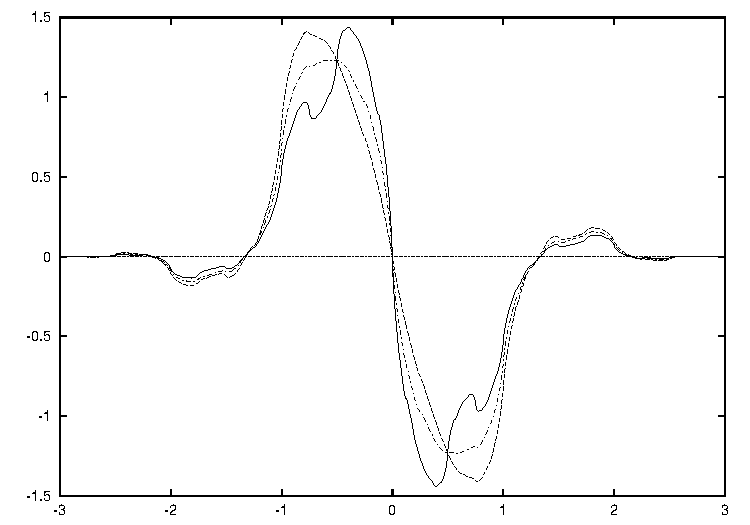
\includegraphics[  width=0.50\paperwidth,
  keepaspectratio]{firstderivative_fund_-0_2_0_15_0}\end{center}


\caption{\label{Figdifffund}Derivatives of the fundamental functions for
$\alpha =-0.2$ (continuous line), $\alpha =0$ (dash-dot line), and
$\alpha =0.15$ (dashed line). The fundamental functions are defined
as the interpolation of $y_{0,k}=\delta _{k,0}$ by the HRS scheme
initialized with the $4-$point Deslauriers-Dubuc dyadic scheme. Derivatives
were estimated using first-order forward finite differences after
8 iterations of the HRS (discarding the placeholders at the last iteration).
The $\alpha =0$ case is in fact the derivative of the Deslauriers-Dubuc
fundamental function.}\end{figure}%


\begin{figure}%
\begin{center}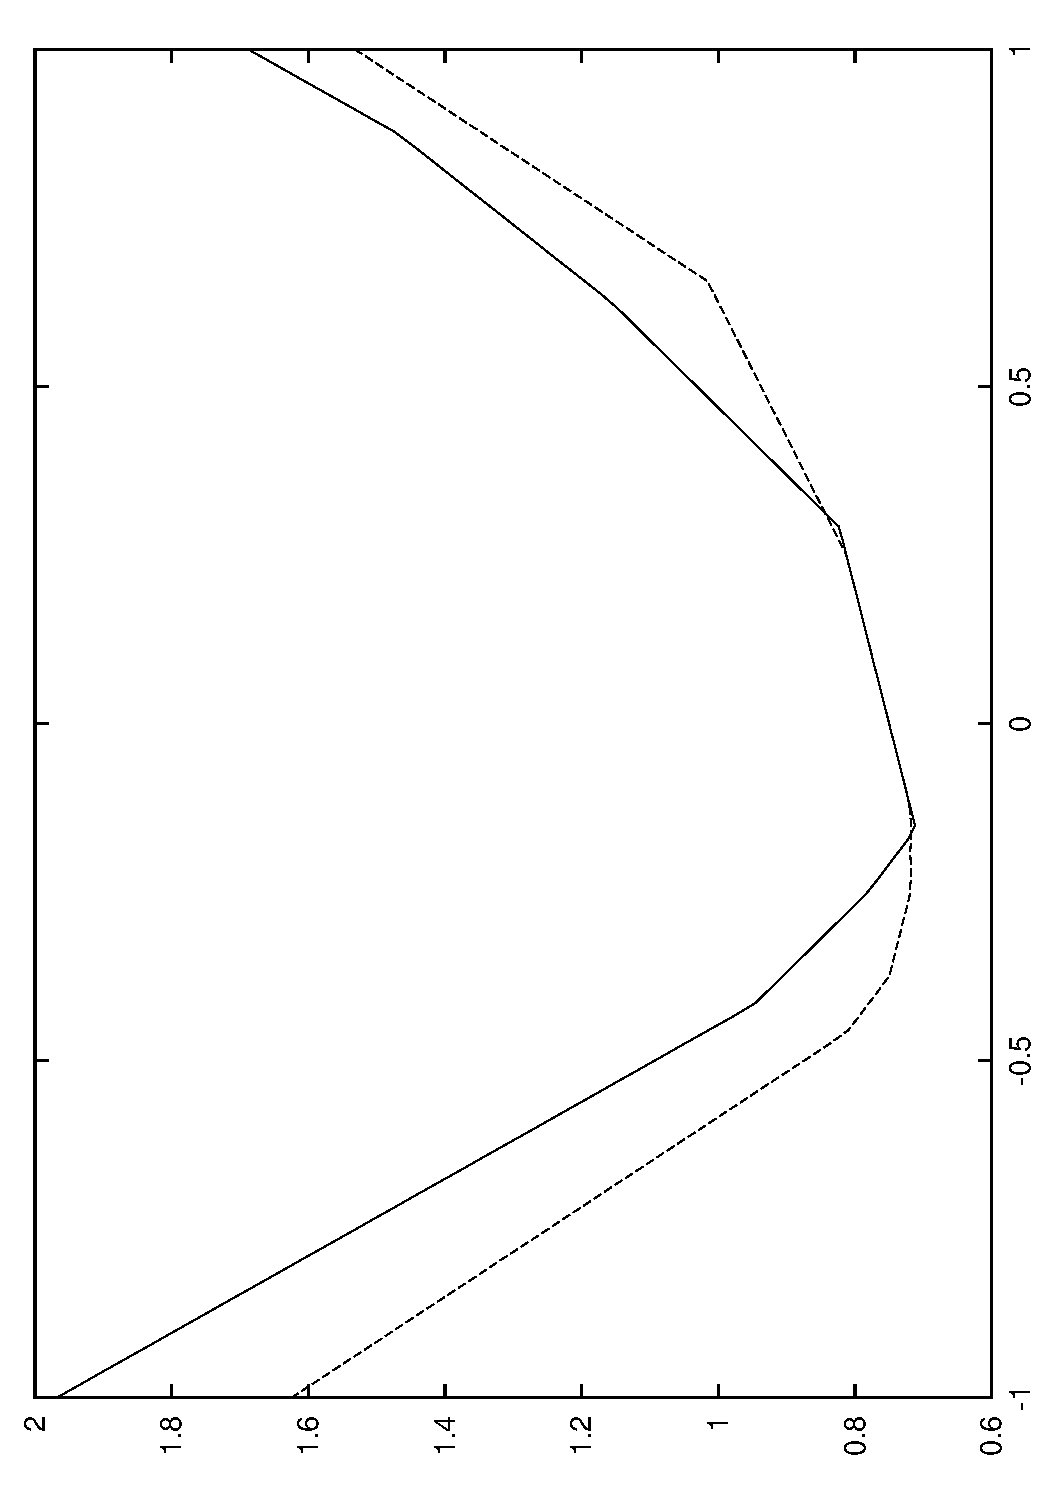
\includegraphics[  height=0.40\paperwidth,
  keepaspectratio,
  angle=270,
  origin=c]{lambdas}\end{center}


\caption{\label{FigLambdas}$\lambda _{1}(\alpha )$ (continuous line) and
$\lambda _{2}(\alpha )$ (dashed line) as in the proof of theorem
\ref{maintheorem}). For a given $\alpha $, an HRS scheme is differentiable
if $\lambda _{HR}(\alpha )=\max \left\{ \lambda _{1}(\alpha ),\lambda _{2}(\alpha )\right\} <1$.}\end{figure}%


Given that the algorithm converges to continuous functions, we can
prove that it must be {}``stable''. In general terms, an algorithm
$R$ is said to be stable if for any data $z$, $|R(z+\delta z)-R(z)|\leq K|\delta z|$
\cite{KuDa}.

\begin{cor}
For $-25/56<\alpha <15/32$, the HRS schemes (algorithm \ref{4pointhrssalgo})
are stable, that is, given $\left|z_{j,k}-\widetilde{z}_{j,k}\right|<\delta \, \forall k\in \Z $
then $\left|z_{j+n,k}-\widetilde{z}_{j+n,k}\right|<K\delta \, \forall k\in \Z $
for all integers $n>0$ and a constant $K$ independent of $\delta $.
\end{cor}
\begin{proof}
Assume we use any $4-$point subdivision scheme as an initialisation
step on the initial data on $z_{j,k},\widetilde{z}_{j,k}$. For $-25/56<\alpha <15/32$,
by theorem \ref{maintheorem}, given the initial data $y_{j,k}=\delta _{k,0}\, \forall k\in \Z $,
we get a continuous ($C^{1}$) interpolation function $F(x)$. Let
$M=\left\Vert F\right\Vert _{L^{\infty }}$, assume $\left|z_{j,k}-\widetilde{z}_{j,k}\right|<\delta \, \forall k\in \Z $,
by linearity, the interpolation function of $z_{j,k}-\widetilde{z}_{j,k}$
is given by $f(x)=\sum _{k=-\infty }^{\infty }\left(z_{j,k}-\widetilde{z}_{j,k}\right)F_{j}\left(x-x_{j,k}\right)$
but since $F$ has compact support $[x_{j,-3},x_{j,3}]$ then $\left\Vert f\right\Vert _{L^{\infty }}\leq 6M\delta $.
It means that the values of the stable nodes are bounded by $-6M\delta $
and $6M\delta $. The placeholders must also be bounded by $6M\delta \sum _{k\in \Z }\left|\gamma _{4k-1}^{DD4}\right|$(see
equation \ref{hrswidguess}).
\end{proof}
\begin{comment}
The author would like to thank S. Dubuc for his help in preparing
the manuscript.

The source code used to generate the figures is available from the
author.
\end{comment}
\begin{thebibliography}{10}
\bibitem{Dau}I. Daubechies, Orthonormal bases of compactly supported wavelets,
Comm. Pure \& Appl. Math. 41, pp. 909--996, 1988.
\bibitem{DeDu}G. Deslauriers and S. Dubuc, Symmetric iterative interpolation processes,
Constr. Approx., 5, pp. 49-68, 1989.
\bibitem{DeDuLe}G. Deslauriers, S. Dubuc, and D. Lemire, Une famille d'ondelettes
biorthogonales sur l'intervalle obtenue par un sch�ma d'interpolation
it�rative, Ann. Sci. Math. Qu�bec 23 no. 1, pp. 37-48, 37-48, 1999.
\bibitem{DuGe}F. Dubeau and R. Gervais, Proc�dures locale et non locale d'interpolation
� l'aide de fonctions splines quadratiques, Ann. Sci. Math. Qu�bec
23 no. 1, pp. 49-61, 1999.
\bibitem{Du}S. Dubuc, Interpolation through an iterative scheme, J. Math. Anal.
Appl., 114, pp. 185-204,1986.
\bibitem{DuLeMe}S. Dubuc, D. Lemire, J.-L. Merrien, Fourier analysis of 2-point Hermite
interpolatory subdivision schemes, J. of Fourier Anal. Appl., 7 no.
5, 2001.
\bibitem{Dyn}N. Dyn, Subdivision schemes in computer-aided geometric design, Advances
in numerical analysis (W. Light, ed.), vol. 2, Clarendon Press, pp.
36-104, 1992.
\bibitem{DyGrLe}N. Dyn, J.A. Gregory, and D. Levin, A 4-point interpolatory subdivision
scheme for curve design. Comput. Aided Geom. Design, 4, pp. 257-268,
1987.
\bibitem{KuDa}F. Kuijt and R. van Damme, Stability of subdivision schemes, Memorandum
no. 1469, Faculty of Applied Mathematics, University of Twente, the
Netherlands.
\bibitem{HaIvDoSa}M.F. Hassan, I.P. Ivrissimitzis, N.A. Dodgson, and M.A. Sabin, An
Interpolating $4-$Point $C^{2}$ Ternary Stationary Subdivision Scheme,
submitted for publication to CAGD (December 18, 2001).
\bibitem{Me92}J.-L. Merrien, A family of Hermite interpolants by bissection algorithms.
Numer. Algorithms 2, pp. 187-200, 1992.
\bibitem{Me99}J.-L. Merrien, Interpolants d'Hermite $C^{2}$ obtenus par subdivision.
M2An Math. Model. Numer. Anal. 33, pp. 55-65, 1999.\end{thebibliography}

\end{document}
